\documentclass[11pt]{article}
\usepackage[margin=0.75in]{geometry}
\usepackage{xcolor}
\usepackage{booktabs}
\usepackage{siunitx}
\usepackage{pgfplots}
\pgfplotsset{compat=1.17}
\usepackage[hidelinks]{hyperref}
\usepackage{titlesec}
\definecolor{accent}{HTML}{1F5C99}
\titleformat*{\section}{\large\bfseries\color{accent}}
\titlespacing*{\section}{0pt}{0.7em}{0.25em}
\setlength{\parindent}{0pt}
\setlength{\parskip}{0.35em}
\pagestyle{empty}

\begin{document}

\begin{center}
  {\LARGE\bfseries\color{accent} Measuring $g$ with a Simple Pendulum}\\[0.35em]
  {\large Experiment 4, PHYS 201 Laboratory}\\[0.45em]
  Alex Rivera \quad | \quad Partner: Jordan Lee \quad | \quad Bench 6\\
  Date performed: 12 March 2026 \quad | \quad Instructor: Dr. M. Okafor
\end{center}

\vspace{0.1em}
{\color{accent}\hrule height 1.2pt}

\section*{Objective}
Determine the local acceleration due to gravity by measuring the period of a
simple pendulum as a function of its length, and compare the result with the
accepted value of \SI{9.81}{\metre\per\second\squared}.

\section*{Apparatus}
Retort stand and clamp, light string, \SI{50}{\gram} brass bob, metre rule
(\SI{\pm 1}{\milli\metre}), digital stopwatch (\SI{\pm 0.01}{\second}),
protractor for setting the release angle below \ang{10}.

\section*{Data}
For each length $L$, the time for 20 oscillations was measured three times and
averaged to obtain the period $T$.

\begin{center}
\begin{tabular}{S[table-format=1.3] S[table-format=2.2] S[table-format=1.3] S[table-format=1.3]}
\toprule
{$L$ (\si{\metre})} & {$t_{20}$ (\si{\second})} & {$T$ (\si{\second})} & {$T^2$ (\si{\second\squared})} \\
\midrule
0.200 & 17.95 & 0.897 & 0.805 \\
0.400 & 25.38 & 1.269 & 1.610 \\
0.600 & 31.10 & 1.555 & 2.418 \\
0.800 & 35.90 & 1.795 & 3.222 \\
1.000 & 40.15 & 2.007 & 4.030 \\
\bottomrule
\end{tabular}
\end{center}

\section*{Results}
Plotting $T^2$ against $L$ gives a straight line through the origin with slope
$4\pi^2/g$.

\begin{center}
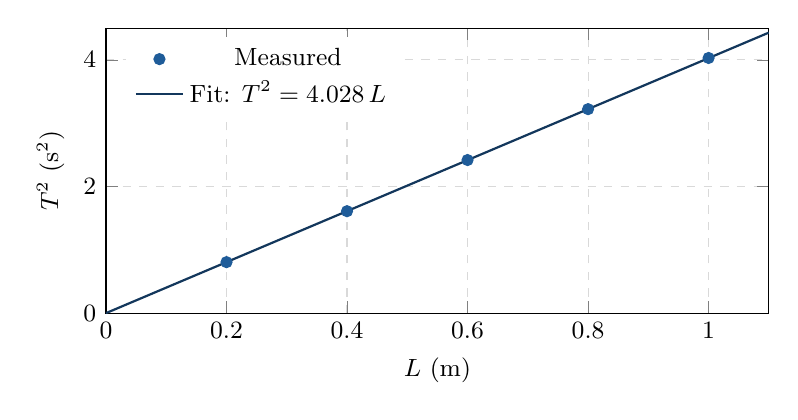
\begin{tikzpicture}
\begin{axis}[
  width=10cm, height=5.2cm,
  xlabel={$L$ (\si{\metre})}, ylabel={$T^2$ (\si{\second\squared})},
  xmin=0, xmax=1.1, ymin=0, ymax=4.5,
  grid=major, grid style={dashed, gray!30},
  legend pos=north west, legend style={draw=none, font=\small},
  tick label style={font=\small}, label style={font=\small},
]
\addplot[only marks, mark=*, color=accent] coordinates {
  (0.200,0.805) (0.400,1.610) (0.600,2.418) (0.800,3.222) (1.000,4.030)
};
\addlegendentry{Measured}
\addplot[thick, color=accent!60!black, domain=0:1.1] {4.028*x};
\addlegendentry{Fit: $T^2 = 4.028\,L$}
\end{axis}
\end{tikzpicture}
\end{center}

The fitted slope of \SI{4.028}{\second\squared\per\metre} yields
$g = 4\pi^2/\text{slope} = \SI{9.80\pm0.06}{\metre\per\second\squared}$,
in agreement with the accepted value to within \SI{0.1}{\percent}.

\section*{Conclusion}
The linear relationship between $T^2$ and $L$ confirms the small-angle
pendulum model. The dominant uncertainty came from reaction time in the
stopwatch measurements, which averaging over 20 oscillations reduced to an
acceptable level.

\end{document}
